
\setcounter{chapter}{5}

\chapter{Flexible representations for word learning}
\label{c:flexible}


Without antedating the discussion of the results of the previous
chapter (this will be happen in Chapter \ref{c:chapter-11}), we want
to highlight two major shortcomings. First, it is a bad strategy to
enumerate many alternative hypotheses about what words mean in the
lexicons of the agents. Because the conceptualized structured meanings
can be any subset of the available categories, referential uncertainty
exponentially increases with the number of categories. Turning this
into an exponentially increasing competition between word meanings
does not scale. Second, the alignment dynamics of the experiments in
the previous chapters contain a bias towards atomic words
meanings. However, in natural language words are not only about single
categories such as red or small but most of them carry complex
structured meanings, a fact that a lexicon representation should be
able to capture.


\begin{figure}[t]
  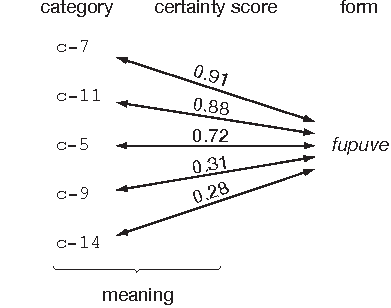
\includegraphics[width=0.41\linewidth]{figures/fwm-word}
  \caption{Illustration of a single flexible word representation. The
    form ``fupuve'' is associated to 5 different categories with
    individual certainty scores. }
\label{f:fwm-word}
\end{figure}


The lexicon formation model introduced in this chapter tries to
address these two shortcomings by capturing uncertainty in the
representation of word meanings themselves\footnote{Some parts of this
  chapter (mainly Section \ref{s:sfwm-representations}) are adapted
  from \cite*{wellens08flexible}, see also
  \cite{wellens07flexible,wellens12multi-dimensional}}. Instead of
having competing mappings to different sets of categories for the same
word, words now have flexible connections to different categories that
are constantly shaped by language use. This is achieved by keeping an
\emph{(un)certainty score} for every category in a form-meaning
association instead of scoring the meanings as a whole (Figure
\ref{f:fwm-word}). This representation is strongly related to both
fuzzy set theory \citep{zadeh65fuzzy} with the degree of membership
interpreted as the degree of (un)certainty, and prototype theory
\citep{rosch73natural}.  Although this representation is identical to
a fuzzy set, in what follows, we refer to the representation as a
\emph{weighted set} to avoid confusion since we will redefine many set
theoretic operations.  By allowing the certainty scores to change, the
representation becomes adaptive and the need to explicitly enumerate
competing hypotheses disappears.




\section{Processing and aligning flexible word representations}
\label{s:sfwm-representations}


Again, the overall strategies for playing language games are identical
to those in the previous two chapters. Also, the same simulated world
from the experiments in the previous chapter is used. Interacting
agents jointly perceive a simulated scene consisting of 2 to 5
objects, which themselves are represented by subsets from a list of 15
categories. We repeat here an example context of such joint perception
from Section \ref{s:sgg-world-simulator} (page
\pageref{s:sgg-world-simulator}):

\centerline{\small\sffamily
  \begin{tabular}{l|l}
    object & categories \\
    \hline
    \texttt{obj-53} & \texttt{c-4  c-2  c-6  c-12  c-9  c-1  c-14  c-5  c-3  c-15  }\\
    \texttt{obj-54} & \texttt{c-10  c-5  c-11  c-9  c-3  c-2  c-8  c-6  c-7  c-14  }\\
    \texttt{obj-55} & \texttt{c-7  c-5  c-6  c-2  c-15  c-8  c-10  c-13  c-4  c-3  }\\
    \texttt{obj-56} & \texttt{c-10  c-2  c-4  c-7  c-1  c-5  c-6  c-3  c-9  c-13  }\\
  \end{tabular}}

~\\

The difference to the experiments in the previous two chapters lies in
the nature of word representations and how they are processed,
invented, adopted and aligned.


\inparagraph{Weighted sets} Perceptions of objects and words in the
lexicon have \emph{weighted sets} as the same underlying
representation. This allows for example production processes to use a
\emph{similarity} measure to find the best combination of words that
expresses a topic. Each weighted set is a list of mappings of a
category (denoted \texttt{category} below) to a real-valued
\emph{certainty score} between $0$ and $1$ (called \texttt{certainty} in
the remainder of this section).

\inparagraph{Similarity between weighted sets} It is possible to
define a weighted similarity measure for the above representation,
taking the certainty scores as weights. Given two weighted sets of
categories as input, the measure returns a real number between $-1$
and $1$, respectively denoting disjunction and equality. This weighted
similarity measure lies at the core of the model and requires detailed
elaboration but we first need to define some additional functions.
Assume a function \texttt{Categories(A)} that takes as input a
weighted set $A$ and returns the normal set $B$ containing only the
categories from $A$, and a function \texttt{CertaintySum(A)} that
takes as input a weighted set $A$ and returns a real number
representing the sum of all the certainty scores.  We can then define
the following operations as slight modifications from those in fuzzy
set theory:

\begin{verbatim+}
\textbf{Function} Intersection(A, B):

\textbf{ForEach} (category \& certainty) \textbf{in} A
    \textbf{If} Find category \textbf{in} Categories(B)
    \textbf{then} Add (category \& certainty) \textbf{to} intersection;
\textbf{End ForEach};

\textbf{Return} intersection;
\end{verbatim+}



\begin{verbatim+}
\textbf{Function} Difference(A, B):

\textbf{ForEach} (category \& certainty) \textbf{in} A
    \textbf{If} not Find category \textbf{in} Categories(B)
    \textbf{then} Add (category \& certainty) \textbf{to} difference
\textbf{End ForEach};

\textbf{Return} difference;
\end{verbatim+}


\noindent Note that in contrast to its definition in fuzzy set theory,
function \texttt{Intersection} is not commutative because it returns
all shared categories between $A$ and $B$ but with certainty scores from
$A$.  With these definitions we can define the weighted similarity
measure as follows:

\begin{verbatim+}
\textbf{Function} Similarity(A, B):

sharedSum $\leftarrow$ CertaintySum(Intersection(A, B)) 
                $\times$ CertaintySum(Intersection(B, A);
diffSum $\leftarrow$ CertaintySum(Difference(A, B) 
              $\times$ CertaintySum(Differenc(B, A));
similarity $\leftarrow$ (sharedSum - diffSum) 
                  / CertaintySum(A) $\times$ CertaintySum(B);

\textbf{Return} similarity;
\end{verbatim+}


\noindent Given two weighted sets $A$ and $B$, \texttt{Similarity} first takes
all shared categories and all disjoint categories between $A$ and $B$. By
using the \texttt{CertaintySum} function we allow the certainty scores
to weight in. It is clear that sharing categories is beneficial for
the similarity and not sharing categories is not. Intuitively,
\texttt{Similarity(A,B)} will be higher the more categories are shared
between $A$ and $B$ and the higher their certainty scores
are. Correspondingly, the more categories are not shared by $A$ and
$B$ and the higher their certainty scores, the lower the result will
be. Some examples:


\begin{verbatim+}
Similarity(((a 1.0) (b 0.5) (c 0.7)), ((a 0.5) (b 0.5) (c 0.7))) 
     = (2.2 $\times$ 1.7 - 0 $\times$ 0) / 2.2 $\times$ 1.7 = 1 
    
Similarity(((a 1) (b 1) (c 1)), ((d 1) (e 1) (f 1))) 
    = (0 $\times$ 0 - 3 $\times$ 3) / 3 $\times$ 3 = -1
    
Similarity(((a 0.9)), ((a 1) (b 0.1) (c 0.2))) 
    = (0.9 $\times$ 1 - 0 $\times$ 0.02) / 0.9 $\times$ 1.3 = 0.77
    
Similarity(((a 0.5) (b 0.5) (c 0.5)), ((a 0.5) (c 0.5) (d 0.5))) 
    = (1 $\times$ 1 - 0.5 $\times$ 0.5) / 1.5 $\times$ 1.5 = 0.33
\end{verbatim+}

\inparagraph{Conceptualization} In the experiments in the previous
chapter, agents conceptualized a scene by finding minimal sets of
categories that \emph{discriminate} the topic from the rest of the
objects in the scene. To allow for more adaptive alignment dynamics,
this now is part of lexicon application. For this, all the objects in
the scene are converted to weighted sets, with constant certainty
scores of $0.5$.

\inparagraph{Production} A speaker that tries to produce gradually
adds words to the utterance so that the combined words are most
similar to the topic and most dissimilar to the other object in the
context:

\begin{verbatim+}
\textbf{Function} Produce(context, topic, lexicon):

bestNewWord $\leftarrow$ nil; \textit{// the current best new candidate word} 
utterance $\leftarrow$ nil; \textit{// The utterance will gradually be combined in here} 
productionScores $\leftarrow$ nil;

\textbf{Loop}
    \textbf{ForEach} word \textbf{in} (lexicon $\setminus$ words in utterance) \textbf{do}
        meaningOfUtterance $\leftarrow$ FuzzySetUnion(\textbf{ForEach} word \textbf{in} utterance
                                            \textbf{collect} Meaning(word));
        meaningOfExtendedUtterance $\leftarrow$ FuzzySetUnion(meaningOfUtterance 
                                                    + Meaning(word));
        objectSimilarities $\leftarrow$ \textbf{ForEach} object \textbf{in} context 
                              \textbf{collect} Similarity(meaningOfExtendedUtterance, 
                                                 object));

        topicSimilarity $\leftarrow$ GetSimilarity(topic, objectSimilarities);
        closestOtherSimilarity $\leftarrow$ Max(objectSimilarities $\setminus$ topicSimilarity);
        Add (topicSimilarity $-$ closestOtherSimilarity) \textbf{to} productionScores;
    \textbf{End ForEach};
    bestNewWord $\leftarrow$ word with highest score in productionScores;
    \textbf{If} ProductionScore(bestCandidate) $>$ average of ProductionScores(utterance)
        \textbf{then} Add bestNewWord \textbf{to} utterance;
        \textbf{Else} \textbf{Break} from Loop;
\textbf{End Loop};

\textbf{Return} utterance;
\end{verbatim+}

\noindent The \texttt{ForEach} loop will fill
\texttt{productionScores} with a score for each unused word in the
lexicon denoting not just its similarity to the topic but taking into
account its similarity to the rest of the context. For example if the
topic is a red object, but all other objects in the context are also
red it doesn't really help that much to use the word red. The
\texttt{bestNewWord} is thus the word with the highest score in
\texttt{productionScores}. If the productionScore for
\texttt{bestNewWord} improves the average of the
\texttt{productionScores} for the \verb+utterance+ so far it gets
added to the \texttt{utterance}, if not the search stops. In the end
\texttt{utterance} is that subset of the lexicon that strikes the
optimal balance between being most similar to the topic and being most
distant from the other objects of the context. This results in context
sensitive multi-word utterances and involves an implicit on-the-fly
discrimination using the lexicon.


\inparagraph{Interpretation} Parsing an utterance amounts to looking
up the meaning of all uttered words, taking the fuzzy union (as
defined in \citealp{zadeh65fuzzy}) of their categories and measuring
similarity between this set and every object in the context:

\begin{verbatim+}
\textbf{Function} Interpret(utterance, context):

interpretedMeaning $\leftarrow$ Fuzzy Union of all meanings for known words in utterance;
objectSimilarities $\leftarrow$ \textbf{ForEach} object \textbf{in} context 
                         \textbf{collect} Similarity(interpretedMeaning, object);
topic $\leftarrow$ object with highest score in objectSimilarities;

\textbf{If} similarityScore of topic $>$ 0
    \textbf{then} \textbf{Return} topic;
\end{verbatim+}

\inparagraph{Invention} After finding the best possible combination of
words to describe the topic, the speaker first interprets his own
utterance himself. In this process -- which is also called
\emph{re-entrance} \citep{steels03re-entrance} -- the speaker takes
himself as a model of the hearer and thus can check potential
misinterpretations, allowing him to rephrase or remedy the
utterance. When re-entrance leads the speaker to a different object
than his own, which means that no combination of words can
discriminate the topic in the current context, refinement of the
lexicon is needed.  The speaker invents a new form and associates to
it, with very low initial certainty score, all so far unexpressed
categories of the topic. Because word meanings can shift, it might not
be necessary to introduce a new word. Chances are that the lexicon
needs a bit more time to be shaped further. Therefore the more similar
the meaning of the utterance is to the topic, the less likely a new
word will be introduced:

\begin{verbatim+}
\textbf{Function} Invention(utterance, topic, context):

interpretedTopic $\leftarrow$ Interpret(utterance, context);
\textbf{If} interpretedTopic $\neq$ topic
\textbf{then}
    interpretedSimilarity $\leftarrow$ Similarity(utterance, interpretedTopic);
    topicSimilarity $\leftarrow$ Similarity(utterance,topic);
    randomNr $\leftarrow$ Random($0$ $1$) \textit{// A random number between 0 and 1}
    \textbf{If} (interpretedSimilarity $-$ topicSimilarity) > randomNr
    \textbf{then} 
        newMeaning $\leftarrow$ Categories of (topic $\setminus$  Meaning(utterance)) 
        newWord $\leftarrow$ makeWord(randomString, newMeaning);
        \textbf{Return} newWord;
\end{verbatim+}


\inparagraph{Adoption} When the hearer encounters one or more novel
words in the utterance, then he needs a way to associate an initial
representation of meaning with the novel forms. For that, the first
interprets the words he knows and tries to play the game without
adopting the novel forms. At the end of the game, when he knows the
topic from communicative feedback, the hearer associates all
unexpressed categories with all novel forms. Just as in invention, the
initial certainty scores start out very low, capturing the uncertainty
of this initial representation. Excluding the categories of the
already known words is the only constraint shaping the initial
representation. Note that there is no explicit enumeration of
competing interpretations:

\begin{verbatim+}
\textbf{Function} Adoption(utterance, topic, novelForms):

newMeaning $\leftarrow$ Categories of (topic $\setminus$  Meaning(utterance))
\textbf{ForEach} form \textbf{in} novelForms \textbf{do} 
    Add makeWord(form, newMeaning) \textbf{to} lexicon; 
\end{verbatim+}


\inparagraph{Alignment} After each interaction, the speaker and hearer
determine which parts of the meanings of the used words were
beneficial (the ones shared with the topic) and which not (the
disjoint categories): 

\begin{verbatim+}
\textbf{Function} Align(agent, topic, utterance)

topicCategories $\leftarrow$ Categories(topic);
sharedCategories $\leftarrow$ Categories(utterance) $\cap$ topicCategories;
disjointCategories $\leftarrow$ Categories(utterance) $\setminus$ topicCategories;
 
\textit{// Update certainty scores}
\textbf{ForEach} word \textbf{in} utterance 
   \textbf{ForEach} category \textbf{in} Meaning(word) 
      \textbf{If} category in sharedCategories
      \textbf{then} IncrementScore(word, category);
      \textbf{Else} DecrementScore(word, category); \textit{// Also removes categories if score < 0} 
\textbf{If} not CommunicatedSuccessfully(agent) 
\textbf{then} \textit{// Make words more specific, only the hearer does this} 
   \textbf{ForEach} word \textbf{in} utterance 
      \textbf{do} Associate disjointCategories to word;
\end{verbatim+}

Certainty scores are slightly shifted every time a word is used in
production or interpretation. The certainty score of the categories
that raised the similarity are incremented (\emph{entrenchment}) and
the others are decremented \emph{erosion}. Categories with a certainty
score equal or less than 0 are removed, resulting in a more general
word meaning. In failed games the hearer adds all unexpressed
categories of the topic, again with very low certainty scores, to all
uttered words, thus making the meanings of those words more specific.



\section{Continuous shaping of word meanings}

\begin{figure}[p]
  \rotatebox{90}
  {
\footnotesize\renewcommand{\arraystretch}{1.35}{
  \begin{tabular}{p{0.4cm}p{1.4cm}p{7cm}p{7cm}p{1.4cm}p{0.6cm}}
    \noalign{\vskip 0.5cm}
  \# & speaker + topic & word meanings speaker & word meanings hearer & hearer + topic & succ. \\
  \hline



500 & agent 7 

\texttt{obj-1495} &\textit{"satitu"} (\texttt{c-2}\textsuperscript{.19}, \texttt{c-1}\textsuperscript{.10}, \texttt{c-3}\textsuperscript{.10}, \texttt{c-13}\textsuperscript{.10}, \texttt{c-5}\textsuperscript{.10}, \texttt{c-6}\textsuperscript{.03}, \texttt{c-8}\textsuperscript{.02}, \texttt{c-4}\textsuperscript{.02}, \texttt{c-11}\textsuperscript{.02})

\textit{"fobigu"} (\texttt{c-7}\textsuperscript{.27}, \texttt{c-5}\textsuperscript{.11}, \texttt{c-8}\textsuperscript{.10}, \texttt{c-4}\textsuperscript{.10}, \texttt{c-11}\textsuperscript{.10}) & \textit{"satitu"} (\texttt{c-8}\textsuperscript{.20}, \texttt{c-5}\textsuperscript{.20}, \texttt{c-2}\textsuperscript{.10}, \texttt{c-1}\textsuperscript{.10})

\textit{"fobigu"} (\texttt{c-7}\textsuperscript{.22}, \texttt{c-8}\textsuperscript{.20}, \texttt{c-4}\textsuperscript{.13}, \texttt{c-3}\textsuperscript{.05}) & agent 3 

 \texttt{obj-1495} & yes \\
501 & agent 1 

\texttt{obj-1497} &\textit{"satitu"} (\texttt{c-5}\textsuperscript{.26}, \texttt{c-1}\textsuperscript{.26}, \texttt{c-11}\textsuperscript{.17}, \texttt{c-4}\textsuperscript{.17}, \texttt{c-10}\textsuperscript{.13}) & \textit{"satitu"} (\texttt{c-5}\textsuperscript{.29}, \texttt{c-8}\textsuperscript{.20}) & agent 6 

 \texttt{obj-1497} & no \\
502 & agent 7 

\texttt{obj-1499} &\textit{"xamexu"} (\texttt{c-8}\textsuperscript{.17}, \texttt{c-14}\textsuperscript{.17}, \texttt{c-12}\textsuperscript{.17}, \texttt{c-15}\textsuperscript{.17})

\textit{"bovaze"} (\texttt{c-8}\textsuperscript{.20}, \texttt{c-5}\textsuperscript{.20}, \texttt{c-9}\textsuperscript{.17}, \texttt{c-1}\textsuperscript{.11})

\textit{"dugobo"} (\texttt{c-6}\textsuperscript{.17}, \texttt{c-1}\textsuperscript{.17}, \texttt{c-3}\textsuperscript{.06}) & \textit{"xamexu"} (\texttt{c-8}\textsuperscript{.20}, \texttt{c-12}\textsuperscript{.17}, \texttt{c-11}\textsuperscript{.04}, \texttt{c-13}\textsuperscript{.02}, \texttt{c-7}\textsuperscript{.02})

\textit{"bovaze"} (\texttt{c-8}\textsuperscript{.32}, \texttt{c-9}\textsuperscript{.32}, \texttt{c-1}\textsuperscript{.24}, \texttt{c-10}\textsuperscript{.02}, \texttt{c-7}\textsuperscript{.02})

\textit{"dugobo"} (\texttt{c-1}\textsuperscript{.20}, \texttt{c-5}\textsuperscript{.10}, \texttt{c-6}\textsuperscript{.10}) & agent 6 

 \texttt{obj-1499} & yes \\
503 & agent 7 

\texttt{obj-1501} &\textit{"satitu"} (\texttt{c-2}\textsuperscript{.14}, \texttt{c-1}\textsuperscript{.13}, \texttt{c-3}\textsuperscript{.13}, \texttt{c-13}\textsuperscript{.13}, \texttt{c-5}\textsuperscript{.13})

\textit{"zepasa"} (\texttt{c-4}\textsuperscript{.17}, \texttt{c-11}\textsuperscript{.13}, \texttt{c-7}\textsuperscript{.07}, \texttt{c-8}\textsuperscript{.07}, \texttt{c-5}\textsuperscript{.04}) & \textit{"satitu"} (\texttt{c-1}\textsuperscript{.39}, \texttt{c-5}\textsuperscript{.30})

\textit{"zepasa"} (\texttt{c-2}\textsuperscript{.13}, \texttt{c-1}\textsuperscript{.13}, \texttt{c-3}\textsuperscript{.10}, \texttt{c-13}\textsuperscript{.10}, \texttt{c-5}\textsuperscript{.10}, \texttt{c-7}\textsuperscript{.07}, \texttt{c-8}\textsuperscript{.07}, \texttt{c-11}\textsuperscript{.02}, \texttt{c-4}\textsuperscript{.02}, \texttt{c-10}\textsuperscript{.02}) & agent 2 

 \texttt{obj-1501} & yes \\
504 & agent 9 

\texttt{obj-1505} &\textit{"mimigo"} (\texttt{c-6}\textsuperscript{.13}) & \textit{"mimigo"} (\texttt{c-7}\textsuperscript{.17}, \texttt{c-8}\textsuperscript{.13}, \texttt{c-2}\textsuperscript{.10}, \texttt{c-4}\textsuperscript{.10}, \texttt{c-3}\textsuperscript{.06}, \texttt{c-12}\textsuperscript{.02}, \texttt{c-13}\textsuperscript{.02}, \texttt{c-11}\textsuperscript{.02}) & agent 4 

 \texttt{obj-1505} & no \\
505 & agent 9 

\texttt{obj-1508} &\textit{"satitu"} (\texttt{c-5}\textsuperscript{.26}, \texttt{c-1}\textsuperscript{.17}, \texttt{c-4}\textsuperscript{.13}, \texttt{c-11}\textsuperscript{.06}, \texttt{c-10}\textsuperscript{.06}, \texttt{c-13}\textsuperscript{.02}, \texttt{c-2}\textsuperscript{.02}) & \textit{"satitu"} (\texttt{c-5}\textsuperscript{.44}, \texttt{c-1}\textsuperscript{.17}, \texttt{c-3}\textsuperscript{.10}, \texttt{c-8}\textsuperscript{.03}) & agent 5 

 \texttt{obj-1508} & yes \\
506 & agent 2 

\texttt{obj-1510} &\textit{"mimigo"} (\texttt{c-3}\textsuperscript{.20}, \texttt{c-7}\textsuperscript{.20}, \texttt{c-2}\textsuperscript{.20}, \texttt{c-8}\textsuperscript{.20}, \texttt{c-4}\textsuperscript{.20}) & \textit{"mimigo"} (\texttt{c-8}\textsuperscript{.17}, \texttt{c-2}\textsuperscript{.13}, \texttt{c-7}\textsuperscript{.10}, \texttt{c-1}\textsuperscript{.10}, \texttt{c-6}\textsuperscript{.10}, \texttt{c-5}\textsuperscript{.10}, \texttt{c-4}\textsuperscript{.02}) & agent 4 

 \texttt{obj-1510} & yes \\
507 & agent 9 

\texttt{obj-1512} &\textit{"guruto"} (\texttt{c-8}\textsuperscript{.47}, \texttt{c-12}\textsuperscript{.47}, \texttt{c-14}\textsuperscript{.34}, \texttt{c-15}\textsuperscript{.34}) & \textit{"guruto"} (\texttt{c-8}\textsuperscript{.41}, \texttt{c-12}\textsuperscript{.34}, \texttt{c-14}\textsuperscript{.19}, \texttt{c-15}\textsuperscript{.12}) & agent 8 

 \texttt{obj-1512} & yes \\
508 & agent 3 

\texttt{obj-1516} &\textit{"tozafu"} (\texttt{c-12}\textsuperscript{.20}, \texttt{c-1}\textsuperscript{.20}, \texttt{c-15}\textsuperscript{.10}, \texttt{c-14}\textsuperscript{.10}) & \textit{"tozafu"} (\texttt{c-8}\textsuperscript{.26}, \texttt{c-7}\textsuperscript{.17}, \texttt{c-12}\textsuperscript{.17}, \texttt{c-9}\textsuperscript{.10}, \texttt{c-10}\textsuperscript{.10}, \texttt{c-1}\textsuperscript{.10}) & agent 1 

 \texttt{obj-1516} & no \\
509 & agent 10 

\texttt{obj-1519} &\textit{"tozafu"} (\texttt{c-2}\textsuperscript{.13}, \texttt{c-8}\textsuperscript{.13}, \texttt{c-9}\textsuperscript{.06}, \texttt{c-6}\textsuperscript{.06}, \texttt{c-5}\textsuperscript{.06}, \texttt{c-15}\textsuperscript{.02}, \texttt{c-12}\textsuperscript{.02}, \texttt{c-14}\textsuperscript{.02}, \texttt{c-1}\textsuperscript{.02}) & \textit{"tozafu"} (\texttt{c-8}\textsuperscript{.23}, \texttt{c-2}\textsuperscript{.07}) & agent 6 

 \texttt{obj-1519} & yes \\
510 & agent 2 

\texttt{obj-1521} &\textit{"zoveza"} (\texttt{c-1}\textsuperscript{.26}, \texttt{c-10}\textsuperscript{.17}, \texttt{c-3}\textsuperscript{.10})

\textit{"fobigu"} (\texttt{c-6}\textsuperscript{.06}, \texttt{c-7}\textsuperscript{.06}, \texttt{c-2}\textsuperscript{.06}) & \textit{"zoveza"} (\texttt{c-1}\textsuperscript{.17}, \texttt{c-7}\textsuperscript{.13}, \texttt{c-6}\textsuperscript{.10}, \texttt{c-5}\textsuperscript{.10}, \texttt{c-2}\textsuperscript{.10}, \texttt{c-8}\textsuperscript{.10}, \texttt{c-3}\textsuperscript{.04}, \texttt{c-10}\textsuperscript{.04})

\textit{"fobigu"} (\texttt{c-3}\textsuperscript{.23}, \texttt{c-7}\textsuperscript{.17}, \texttt{c-4}\textsuperscript{.07}) & agent 4 

 \texttt{obj-1521} & yes \\
511 & agent 7 

\texttt{obj-1523} &\textit{"fobigu"} (\texttt{c-7}\textsuperscript{.30}, \texttt{c-5}\textsuperscript{.14}, \texttt{c-8}\textsuperscript{.02}, \texttt{c-4}\textsuperscript{.02}, \texttt{c-11}\textsuperscript{.02}) & \textit{"fobigu"} (\texttt{c-4}\textsuperscript{.36}, \texttt{c-7}\textsuperscript{.23}, \texttt{c-8}\textsuperscript{.23}, \texttt{c-2}\textsuperscript{.13}, \texttt{c-3}\textsuperscript{.13}) & agent 9 

 \texttt{obj-1523} & no \\
512 & agent 9 

\texttt{obj-1525} &\textit{"fobigu"} (\texttt{c-4}\textsuperscript{.31}, \texttt{c-7}\textsuperscript{.25}, \texttt{c-8}\textsuperscript{.17}, \texttt{c-3}\textsuperscript{.17}, \texttt{c-5}\textsuperscript{.10}, \texttt{c-1}\textsuperscript{.10}, \texttt{c-10}\textsuperscript{.10}, \texttt{c-2}\textsuperscript{.07})

\textit{"zepasa"} (\texttt{c-7}\textsuperscript{.26}, \texttt{c-8}\textsuperscript{.26}, \texttt{c-4}\textsuperscript{.07}) & \textit{"fobigu"} (\texttt{c-6}\textsuperscript{.10}, \texttt{c-7}\textsuperscript{.10})

\textit{"zepasa"} (\texttt{c-2}\textsuperscript{.17}, \texttt{c-1}\textsuperscript{.17}, \texttt{c-13}\textsuperscript{.13}, \texttt{c-5}\textsuperscript{.13}, \texttt{c-4}\textsuperscript{.06}, \texttt{c-3}\textsuperscript{.02}, \texttt{c-7}\textsuperscript{.02}, \texttt{c-8}\textsuperscript{.02}) & agent 2 

 \texttt{obj-1525} & yes \\
513 & agent 4 

\texttt{obj-1529} &\textit{"guruto"} (\texttt{c-12}\textsuperscript{.35}, \texttt{c-8}\textsuperscript{.35}, \texttt{c-15}\textsuperscript{.19}, \texttt{c-14}\textsuperscript{.19}) & \textit{"guruto"} (\texttt{c-8}\textsuperscript{.23}, \texttt{c-15}\textsuperscript{.20}, \texttt{c-12}\textsuperscript{.20}, \texttt{c-14}\textsuperscript{.20}) & agent 5 

 \texttt{obj-1529} & yes \\
514 & agent 1 

\texttt{obj-1532} &\textit{"bovaze"} (\texttt{c-7}\textsuperscript{.13}, \texttt{c-8}\textsuperscript{.13}, \texttt{c-1}\textsuperscript{.13}, \texttt{c-10}\textsuperscript{.13}, \texttt{c-9}\textsuperscript{.13}) & \textit{"bovaze"} (\texttt{c-8}\textsuperscript{.23}, \texttt{c-9}\textsuperscript{.20}, \texttt{c-5}\textsuperscript{.14}, \texttt{c-1}\textsuperscript{.05}) & agent 7 

 \texttt{obj-1532} & yes \\

\noalign{\vskip 1cm}   
\end{tabular}}
}
  \caption{Overview of 15 consecutive interactions in a population of
    10 agents from game 500 on. It shows the speaker with his chosen
    topic, the words used by the speaker with their associated
    meanings (the certainty scores are in superscript), the word
    meanings interpreted by the hearer, the hearer and the interpreted
    topic, and whether the agents reached communicative success.}
  \label{f:sfwm-trace}
\end{figure}



When using this similarity based lexicon application, word meanings
become immediately useful. As shown in Figure \ref{f:sfwm-trace}, the
agents of the population have very different notions of what each word
means in the beginning, but nevertheless they communicate very
successfully from this early on. This is because words are understood
even when most of their meanings are not conventionalized -- it is
enough to reach a successful interpretation of an utterance when the
similarity of the words to the topic is the highest among all the
referents. 

For example in the first shown interaction 500, the speaker associates
9 different categories to the form ``satitu'', whereas the hearer
connects only 4 categories to it. Furthermore, only the two categories
\texttt{c-2} and \texttt{c-5} are shared between the tho agents, and
nevertheless they are able to communicate successfully. Stretching
existing word meanings so to rather unconventional uses in production
and broadly applying words in interpretation (i.e. the ability to use
linguistic items beyond their core meanings) is what
\cite{langacker00dynamic} calls \emph{extension}.

This flexible word application also clearly shows the other
interactions in Figure \ref{f:sfwm-trace}. Although speakers and
hearers often have some shared categories in the words that they use,
most of the time word meanings drastically differ, both in the
categories and certainty scores themselves but also in the specificity
of words. For example in interaction 509, the speaker associates 9
categories to the form ``tozafu'', whereas the speaker only connects
two categories to it.

\begin{figure}[p]
  \begin{tabular}{c}
    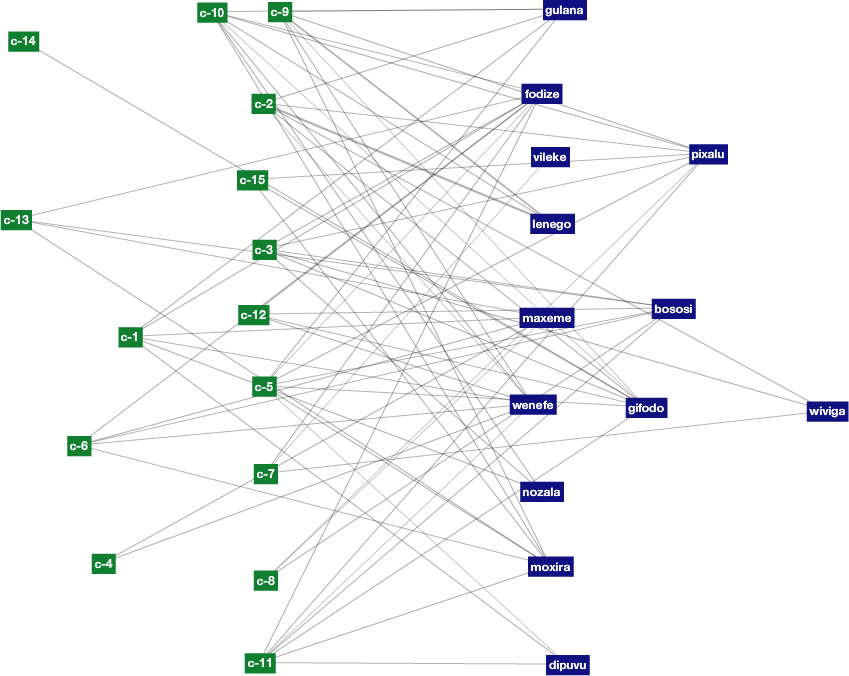
\includegraphics[width=0.73\textwidth]{figures/sfwm-lexicon-500} \\
    \\
    \\
    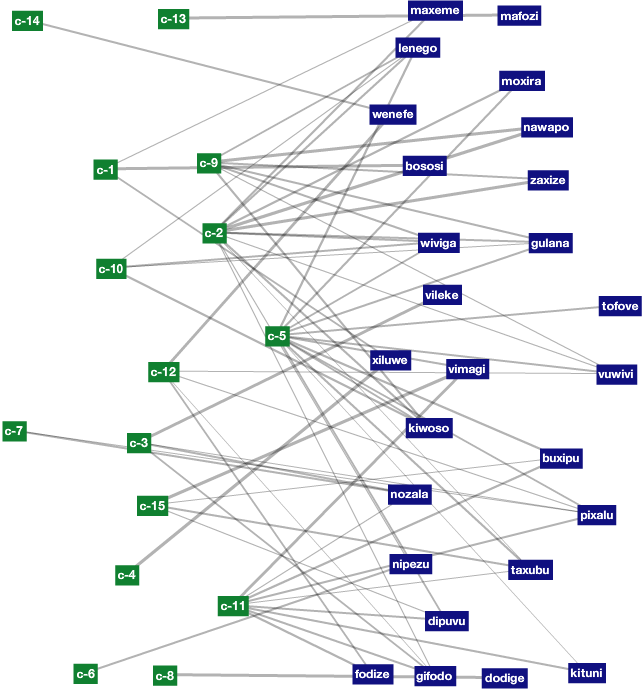
\includegraphics[width=0.55\textwidth]{figures/sfwm-lexicon-10000} \\
    \\
  \end{tabular}
  \caption{A network visualization of the lexicon of a single agent at
    interaction 500 (top) and interaction 10000 (bottom). For each
    word denoted by its form, all categories that are associated to
    the form are shown. The line width represents the certainty scores
    of these associations.  }
  \label{f:sfwm-semiotic-network}
\end{figure}

Nevertheless, agents communicate already successfully in the majority
of the shown early interactions. Interestingly (and very different
from the experiments in the previous chapter), agents that use
multiple words in an utterances are more likely to reach their
communicative goal than agents that use only single words. For example
in interaction 502, the speaker uses the three different words
``xamexu'', ``bovaze'' and ``dugobo'', and although the hearer has a
very different understanding what these words mean, the interaction
results in a communicative success. The reason for this is that using
more words doesn't increase the danger of using them in a wrong
``wrong'' way as in the experiments before, but quite to the contrary
adds to the chances of being understood by being more expressive. When
words are not very conventionalized yet but some coherence exists,
then the more words are used, the higher the chance that the overall
similarity to the similarity to objects in the context selects the
correct topic.



\startfiguregroup

\begin{figure}[t]
  
{\footnotesize\renewcommand{\arraystretch}{1.5}
\begin{tabular}{@{}p{1.2cm}|p{1.3cm}@{}p{0.8cm}@{}|p{1.3cm}@{}p{0.8cm}@{}|p{1.3cm}@{}p{0.8cm}@{}|p{1.3cm}@{}p{0.8cm}@{}}
form & agent 1 &  & agent 2 &  & agent 3 &  & agent 4 & \\
\hline
\textit{"sidigu"} & \texttt{c-8}

\texttt{c-6}

\texttt{c-5}

\texttt{c-7}

\texttt{c-3} & 0.34

0.34

0.26

0.17

0.17 & \texttt{c-6}

\texttt{c-8}

\texttt{c-5}

\texttt{c-3}

\texttt{c-4}

\texttt{c-1} & 0.32

0.17

0.17

0.09

0.05

0.04 & \texttt{c-6}

\texttt{c-7}

\texttt{c-3}

\texttt{c-8}

\texttt{c-5} & 0.20

0.20

0.10

0.10

0.10 & \texttt{c-8}

\texttt{c-3}

\texttt{c-5}

\texttt{c-2}

\texttt{c-6} & 0.39

0.32

0.32

0.17

0.09\\
\hline
\textit{"wefugu"} & \texttt{c-8}

\texttt{c-7}

\texttt{c-1}

\texttt{c-2}

\texttt{c-12}

\texttt{c-9}

\texttt{c-5} & 0.30

0.22

0.13

0.02

0.02

0.02

0.02 & \texttt{c-8} & 0.13 & \texttt{c-1}

\texttt{c-2}

\texttt{c-11}

\texttt{c-8}

\texttt{c-7}

\texttt{c-6}

\texttt{c-15}

\texttt{c-4} & 0.13

0.13

0.10

0.10

0.10

0.02

0.02

0.02 & \texttt{c-4}

\texttt{c-7}

\texttt{c-11}

\texttt{c-6} & 0.17

0.17

0.02

0.02\\
\hline
\textit{"vufaxe"} & \texttt{c-5}

\texttt{c-9}

\texttt{c-2}

\texttt{c-12} & 0.43

0.25

0.14

0.08 & \texttt{c-5}

\texttt{c-9}

\texttt{c-12}

\texttt{c-14} & 0.38

0.35

0.20

0.11 & \texttt{c-5}

\texttt{c-9}

\texttt{c-12}

\texttt{c-2} & 0.57

0.40

0.17

0.15 & \texttt{c-9}

\texttt{c-2}

\texttt{c-5}

\texttt{c-12}

\texttt{c-14} & 0.30

0.30

0.14

0.06

0.06\\
\hline
\textit{"bivura"} & \texttt{c-8}

\texttt{c-7}

\texttt{c-1}

\texttt{c-2}

\texttt{c-4}

\texttt{c-5}

\texttt{c-3} & 0.24

0.19

0.17

0.14

0.09

0.06

0.06 & \texttt{c-5}

\texttt{c-9}

\texttt{c-1}

\texttt{c-14}

\texttt{c-12}

\texttt{c-6}

\texttt{c-8}

\texttt{c-7} & 0.31

0.11

0.10

0.10

0.10

0.09

0.06

0.06 & \texttt{c-3}

\texttt{c-7}

\texttt{c-4}

\texttt{c-1}

\texttt{c-8}

\texttt{c-5}

\texttt{c-2} & 0.17

0.17

0.13

0.13

0.07

0.07

0.02 & \texttt{c-7} & 0.20\\
\hline
\textit{"kunite"} & \texttt{c-5}

\texttt{c-6}

\texttt{c-9}

\texttt{c-10}

\texttt{c-2}

\texttt{c-8}

\texttt{c-7}

\texttt{c-3} & 0.13

0.13

0.10

0.10

0.10

0.10

0.02

0.02 & \texttt{c-9}

\texttt{c-5}

\texttt{c-7}

\texttt{c-3}

\texttt{c-4}

\texttt{c-1}

\texttt{c-6}

\texttt{c-2} & 0.10

0.10

0.10

0.10

0.06

0.06

0.06

0.06 & \texttt{c-2}

\texttt{c-4}

\texttt{c-5}

\texttt{c-3}

\texttt{c-1} & 0.20

0.13

0.10

0.10

0.10 & \texttt{c-5}

\texttt{c-1}

\texttt{c-3}

\texttt{c-4}

\texttt{c-2}

\texttt{c-10}

\texttt{c-8} & 0.13

0.10

0.10

0.10

0.10

0.02

0.02
\end{tabular}}

  \caption{Word meanings maintained first four agents of a population
    of 10 for the first 5 forms after 500 interactions. Word
    representations are shown with their association scores to
    different meanings (compared to previous similar charts where
    competing word meanings were shown). }
  \label{f:sfwm-lexicon-forms-500}
\end{figure}

\begin{figure}[t]
  
{\renewcommand{\arraystretch}{1.5}
\begin{tabular}{@{}p{1.2cm}|p{1.3cm}@{}p{0.8cm}@{}|p{1.3cm}@{}p{0.8cm}@{}|p{1.3cm}@{}p{0.8cm}@{}|p{1.3cm}@{}p{0.8cm}@{}}
form & agent 1 &  & agent 2 &  & agent 3 &  & agent 4 & \\
\hline
\textit{"sidigu"} & \texttt{c-8}

\texttt{c-5}

\texttt{c-3}

\texttt{c-6} & 0.68

0.59

0.57

0.48 & \texttt{c-8}

\texttt{c-5}

\texttt{c-3}

\texttt{c-6} & 0.60

0.57

0.55

0.33 & \texttt{c-5}

\texttt{c-8}

\texttt{c-3}

\texttt{c-6} & 0.66

0.63

0.59

0.46 & \texttt{c-8}

\texttt{c-5}

\texttt{c-3}

\texttt{c-6}

\texttt{c-2} & 0.73

0.68

0.50

0.43

0.16\\
\hline
\textit{"wefugu"} & \texttt{c-7}

\texttt{c-8}

\texttt{c-1} & 0.60

0.56

0.21 & \texttt{c-7}

\texttt{c-8}

\texttt{c-4}

\texttt{c-2}

\texttt{c-1} & 0.64

0.51

0.44

0.36

0.32 & \texttt{c-4}

\texttt{c-2}

\texttt{c-8}

\texttt{c-7}

\texttt{c-1} & 0.59

0.46

0.45

0.45

0.26 & \texttt{c-8}

\texttt{c-7}

\texttt{c-4}

\texttt{c-2}

\texttt{c-1} & 0.55

0.53

0.46

0.40

0.13\\
\hline
\textit{"vufaxe"} & \texttt{c-5}

\texttt{c-9} & 0.80

0.44 & \texttt{c-5}

\texttt{c-9}

\texttt{c-12} & 0.77

0.73

0.27 & \texttt{c-5}

\texttt{c-9}

\texttt{c-12} & 0.84

0.67

0.29 & \texttt{c-9}

\texttt{c-5}

\texttt{c-12} & 0.74

0.72

0.22\\
\hline
\textit{"bivura"} & \texttt{c-3}

\texttt{c-5}

\texttt{c-6}

\texttt{c-8}

\texttt{c-7} & 0.53

0.53

0.51

0.38

0.31 & \texttt{c-3}

\texttt{c-7}

\texttt{c-5}

\texttt{c-6}

\texttt{c-8} & 0.70

0.64

0.55

0.54

0.48 & \texttt{c-3}

\texttt{c-5}

\texttt{c-7}

\texttt{c-8}

\texttt{c-6} & 0.67

0.67

0.37

0.32

0.31 & \texttt{c-5}

\texttt{c-3}

\texttt{c-6}

\texttt{c-8}

\texttt{c-7} & 0.61

0.58

0.50

0.36

0.29\\
\hline
\textit{"rotapo"} & \texttt{c-2}

\texttt{c-5} & 0.80

0.53 & \texttt{c-2}

\texttt{c-5} & 0.83

0.54 & \texttt{c-2}

\texttt{c-5}

\texttt{c-3} & 0.86

0.46

0.03 & \texttt{c-2}

\texttt{c-5} & 0.82

0.54
\end{tabular}}

  \caption{Word meanings for the same 4 agents as in Figure
    \ref{f:sfwm-lexicon-forms-500} above, but 4500 interactions later
    (at interaction 5000).}
  \label{f:sfwm-lexicon-forms-5000}
\end{figure}

\stopfiguregroup


\startfiguregroup

\begin{figure}[t]
  \gnuplotfigure{figures/sfwm-attribute-scores-1}
  \caption{Slowly adapting word meanings of a single word of a single
    agent over time. The certainty scores of the associations of the
    form ``lonigo'' to its categories are shown over the course of
    16000 interactions. Not that each agent only takes part in every
    fifth interaction on average. }
  \label{f:sfwm-attribute-scores-1}
\end{figure}

\begin{figure}[t]
  \gnuplotfigure{figures/sfwm-attribute-scores-3}
  \caption{Adapting word meanings of another word over time.}
  \label{f:sfwm-attribute-scores-2}
\end{figure}

\begin{figure}[t]
  \gnuplotfigure{figures/sfwm-attribute-scores-2}
  \caption{Adapting word meanings of yet another word over time.}
  \label{f:sfwm-attribute-scores-3}
\end{figure}

\stopfiguregroup


~\\

\noindent In addition to the flexible lexicon application, the
similarity-based alignment mechanisms are the second key factor for
the dynamics of this lexicon formation model. Instead of deleting
competing hypotheses on word meanings from their lexicons, agents
gradually refine and shift the meanings of their words to better
conform future uses.  Figure \ref{f:sfwm-semiotic-network} shows a
network representation of a single agent's lexicon at interaction 500
and then at interaction 10000. Compared to the similar Figure
\ref{f:sgg-mw-structured-lexicon-500} (page
\pageref{f:sgg-mw-structured-lexicon-500}) from the last chapter for
the same simulated environment, there are much less word forms in the
lexicon after 500 interactions. During the next 9500 interaction, this
agent carefully entrenches his association scores (denoted by the line
widths). Whereas in the beginning words forms are associated to many
categories, words later become more specialized and associate less
categories with higher scores. As a consequence, more words enter the
lexicon as the existing words cover fewer potential meanings. Also
different from the previous competition based dynamics, most of the
word forms from the lexicon at interaction are still around at
interaction 10000.

Analogously, Figures \ref{f:sfwm-lexicon-forms-500} and
\ref{f:sfwm-lexicon-forms-5000} further illustrate the same effects by
showing the categories and association scores for the first 5 forms
for the 4 agents out of a population of 10 agents at 500 and 5000
interactions. Furthermore, Figures
\ref{f:sfwm-attribute-scores-1}--\ref{f:sfwm-attribute-scores-3} show
three typical evolutions of words of a single agent. In Figure
\ref{f:sfwm-attribute-scores-1}, the form ``lonigo'' gets associated
to 8 different categories within the first 4000 interactions. From
very early on, the two categories \texttt{c-1} and \texttt{c-2} become
dominant and from interaction 4000 on, all other categories become
eliminated and the certainty scores for \texttt{c-1} and \texttt{c-2}
continuously increase. For the form ``duropi'' (Figure
\ref{f:sfwm-attribute-scores-2}), it takes a bit longer to find it's
later meaning. After around 3000 interactions, the three categories
\texttt{c-1}, \texttt{c-2} and \texttt{c-4} emerge, of which
\texttt{c-2} has difficulties to become conventionalized and
eventually disappears shortly after interaction 12000. That particular
word is therefore an example of a word that changes its specificity
from being more specific (covering three categories) to more general
(covering two categories). An example for the contrary is the word
``lonigo'' in Figure \ref{f:sfwm-attribute-scores-3}. This one starts
out being very general (covering only the single category
\texttt{c-7}) and later on acquires more meanings (\texttt{c-3} at
interaction 5000 and \texttt{c-2} at interaction 8000), thus becoming
more specific.


\startfiguregroup

\begin{figure}[t]
  \gnuplotfigure{figures/sfwm-success+lexicon-size+coherence}
  \caption{Comm\-unicative success (measure
    \ref{m:communicative-success}), lexicon size (measure
    \ref{m:lexicon-size}) and lexicon coherence (measure
    \ref{m:fwm-lexicon-coherence}) in a population of 10 agents averaged
    over 10 repeated series of 16000 language games. Each measure is
    averaged over the last 250 interactions. }
  \label{f:sfwm-success+lexicon-size+coherence}
\end{figure}


\begin{figure}[t]
  \gnuplotfigure{figures/sfwm-lexicon}
  \caption{The distance of the utterance to the topic (measure
    \ref{m:fwm-distance-utterance-topic}), the average number of
    categories covered per word (measure
    \ref{m:fwm-attributes-per-word}) and the average utterance length
    (measure \ref{m:utterance-length}) are averaged over 10 repeated
    series of 16000 language games}
  \label{f:sfwm-lexicon}
\end{figure}

\stopfiguregroup


\begin{measure}[b]{Lexicon coherence between speaker and
    hearer II}{m:fwm-lexicon-coherence}
  Provides a measure for how similar the lexicons of the interacting
  agents are. After each interaction, the similarity between the
  lexicons of the speaker and the hearer is computed as the average of
  the output of the \texttt{similarity} function for each word form
  that both agents have in their lexicon and of $0$ for all others.

~\\

  Again, the lexicon similarity between speaker and hearer is only an
  approximation of the population coherence, but is used because its
  is much more efficiently computed than a measure that involves
  comparing the lexicons of all agents.
\end{measure}


\begin{measure}[b]{Distance utterance to topic}{m:fwm-distance-utterance-topic}
  Measures how well the words of the utterance cover the topic. After
  each interaction, the average of the \texttt{similarity} function is
  computed between all words used by the speaker and the
  utterance. Results are averaged over the last 250 interactions.
\end{measure}


\begin{measure}[b]{Average number of categories per
    word}{m:fwm-attributes-per-word}
  Measures how specific words are. For all words in an agents lexicon,
  the average number of categories that are associated to a form with
  a non-zero certainty score is computed. Results are averaged over
  all agents of the population and the last 250 interactions.
\end{measure}



~\\

\noindent Finally, the overall alignment dynamics for agents that use
flexible word representations and learning mechanisms are shown in
Figure \ref{f:sfwm-success+lexicon-size+coherence}. Compared to Figure
\ref{f:sgg-mw-structured-success+lexicon-size} on page
\pageref{f:sgg-mw-structured-success+lexicon-size}, two things are
clearly visible. First, agents start communicating successfully from a
bit earlier on but more importantly, never reach 100 percent
communicative success. This is due to the fact that agents often
stretch their existing words in order to apply in difficult contexts
instead of inventing new words, which is interpreted differently by
hearers in about two percent of the cases. Second, the typical
bell-curved evolution of lexicon size does not occur at all. Instead
of inventing and adopting lots of words in the beginning and pruning
them later on, agents grow their lexicons much more
conservatively. Most of the words enter the lexicons in the first few
thousand interactions, but even new words emerge as the lexicons
specialize.

Additionally, Figure \ref{f:sfwm-lexicon} investigates word usage in
more depth. First, the overall distance of the words in the utterance
to the the topic decreases from 1 in the beginning to almost 0.5
(complete category overlap), showing that agents indeed manage to
shape their words to be more applicable in future
conversations. Second, the average number of categories covered per
word decreases from about 5 to a stable level of 3.5 as part of the
entrenchment process. This shows that the word representations are
suitable for maintaining structured word meanings, which was not the
case for the competition based models from the previous chapter
because they contained a frequency-bias towards atomic word meanings.



\section{Robust scaling dynamics}

\startfiguregroup

\begin{figure}[p]
  \gnuplotfigure{figures/sfwm-communicative-success-vs-population-size}
  \caption{Communi\-cative success (measure
    \ref{m:communicative-success}) for five different population
    sizes. Results are averaged over 10 series of varying length, but
    each with 8000 interactions per agent.}
  \label{f:sfwm-communicative-success-vs-population-size}
\end{figure}

\begin{figure}[p]
  \gnuplotfigure{figures/sfwm-lexicon-size-vs-population-size}
  \caption{Lexicon size (measure \ref{m:lexicon-size}) for five
    different population sizes. Results are averaged over 10 series of
    varying length, but each with 8000 interactions per agent.}
  \label{f:sfwm-lexicon-size-vs-population-size}
\end{figure}

\begin{figure}[p]
  \gnuplotfigure{figures/sfwm-lexicon-coherence-vs-population-size}
  \caption{Lexicon coherence (measure \ref{m:fwm-lexicon-coherence})
    for five different population sizes. Results are averaged over 10
    series of varying length, but each with 8000 interactions per
    agent.}
  \label{f:sfwm-lexicon-coherence-vs-population-size}
\end{figure}


\stopfiguregroup

To demonstrate that the lexicon formation model introduced in this
chapter also performs well when the complexity of the interaction
scenario increases, we repeat the scaling studies from the previous
Chapter (see Section \ref{s:sgg-mv-structured-scaling}, page
\pageref{s:sgg-mv-structured-scaling}).

~\\



\startfiguregroup

\begin{figure}[p]
  \gnuplotfigure{figures/sfwm-context-size-vs-communicative-success}
  \caption{Communi\-cative success (measure
    \ref{m:communicative-success}) for world simulators with
    increasing number of objects per scene. Results are averaged over
    10 series of 80000 interactions. }
  \label{f:sfwm-context-size-vs-communicative-success}
\end{figure}


\begin{figure}[p]
  \gnuplotfigure{figures/sfwm-context-size-vs-lexicon-coherence}
  \caption{Lexicon coherence (measure \ref{m:fwm-lexicon-coherence})
    for world simulators with increasing number of objects per
    scene. Results are averaged over 10 series of 80000
    interactions. }
  \label{f:sfwm-context-size-vs-lexicon-coherence}
\end{figure}


\begin{figure}[p]
  \gnuplotfigure{figures/sfwm-context-size-vs-lexicon-size}
  \caption{Lexicon size (measure \ref{m:lexicon-size})
    for world simulators with increasing number of objects per
    scene. Results are averaged over 10 series of 80000
    interactions. }
  \label{f:sfwm-context-size-vs-lexicon-size}
\end{figure}

\stopfiguregroup

\noindent First, Figures
\ref{f:sfwm-communicative-success-vs-population-size}--\ref{f:sfwm-lexicon-coherence-vs-population-size}
present the main alignment dynamics for increasing population sizes of
up to 100 agents. It clearly shows that the model scales well with the
number of agents in the population. Agents communicate successfully
from very early on and high levels of coherence are reached in all
conditions. This is in stark contrast to the same analysis for the
models in the previous chapter (see Figure
\ref{f:sgg-mw-structured-best-best-population-size-vs-communicative-success}),
where agents needed to go through thousands of interactions of random
search without any success whatsoever. Furthermore, the average
lexicon size increases with bigger populations because more words get
independently invented and adapted by the population. Since there is
no explicit mechanism for synonymy damping, these words stay in the
population and specialize on more specific meanings.


A growing number of objects per scene has almost no effect
on the dynamics of the game (see Figures
\ref{f:sfwm-context-size-vs-communicative-success}--\ref{f:sfwm-context-size-vs-lexicon-size}).
This is because more alternative conceptualizations of a scene do not
result in a higher hypothesis space that needs to be explored but
instead only puts a little more burden on the similarity based lexicon
application.

\startfiguregroup

\begin{figure}[t]
  \gnuplotfigure{figures/sfwm-number-of-attributes-vs-communicative-success}
  \caption{Communi\-cative success (measure
    \ref{m:communicative-success}) for world simulators with
    increasing number of available categories. Results are averaged over 10
    series of 80000 interactions. }
  \label{f:sfwm-number-of-attributes-vs-communicative-success}
\end{figure}

\begin{figure}[t]
  \gnuplotfigure{figures/sfwm-number-of-attributes-vs-lexicon-size}
  \caption{Lexicon size (measure \ref{m:lexicon-size}) for world
    simulators with increasing number of available categories. Results
    are averaged over 10 series of 80000 interactions. }
  \label{f:sfwm-number-of-attributes-vs-lexicon-size}
\end{figure}

\begin{figure}[t]
  \gnuplotfigure{figures/sfwm-number-of-attributes-vs-lexicon-coherence}
  \caption{Lexicon coherence (measure \ref{m:fwm-lexicon-coherence})
    for world simulators with increasing number of available
    categories. Results are averaged over 10 series of 80000
    interactions. }
  \label{f:sfwm-number-of-attributes-vs-lexicon-coherence}
\end{figure}

\stopfiguregroup

And finally, Figures
\ref{f:sfwm-number-of-attributes-vs-communicative-success}--\ref{f:sfwm-number-of-attributes-vs-lexicon-coherence}
show what happens when the number of categories in the world
simulation increases. More categories mean that agents invent more
words and thus it takes longer to align their meanings, but
nevertheless the model copes well with an increasing meaning space.




%%% Local Variables: 
%%% mode: latex
%%% TeX-master: "phdbook"
%%% End: 
